% Encoding: UTF-8

\section{Angriffsszenarien}\label{sec:angriffszenarien}

\begin{figure}
    \centering
    \begin{subfigure}[b]{0.3\textwidth}
        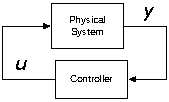
\includegraphics[width=\textwidth]{abstrakt}
        \caption{Ohne Angriffspunkte}
        \label{fig:abstrakt}
    \end{subfigure}
    \qquad
    \begin{subfigure}[b]{0.4\textwidth}
        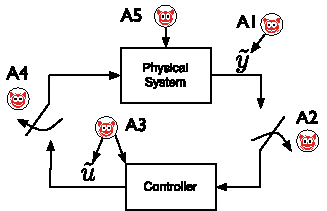
\includegraphics[width=\textwidth]{attack_points}
        \caption{Mit Angriffspunkten}
        \label{fig:attack_points}
    \end{subfigure}
    \caption{Abstraktion eines \cps~\cite{CAS08}}
\end{figure}

In Abbildung~\ref{fig:abstrakt} ist eine abstrakte Darstellung eines \cps zu sehen.
Der \enquote{Controller} sendet Befehle über u an das \enquote{Physical System}.
Dieses wiederum schickt Resultate oder Sensorwerte über y an den \enquote{Controller}.
In Abbildung~\ref{fig:attack_points} sind mögliche Angriffspunkte dargestellt.
Hierbei stellen A1 und A2 Täuschungsangriffe dar, A4 und A2 \gls{dos} und A5 einen physischen Angriff.
Im folgenden Kapitel sollen Angriffe an den verschiedenen Punkten des \cps dargestellt werden.

% Sabotage und Spionage
% Punkte wo angegriffen werden kann (Fink, Figure 1.1) (Cardenas 2008, Figure 3)
% Migration von Legacy Systemen ist kritisch (Gollman, 1.)
% Unterschied zu Cybersystemen (Cardenas 2008, 3.)
% IoT Unterschiede zu Cybersystemen (FPA+18)
% Workflow von CPS (WYX+10, II.)
\subsection{\glsentrytext{dos} Angriff}\label{subsec:dos}
% Availability

\gls{dos} Angriffe Zielen darauf ab das Cybersystem mit einer großen Flut an Informationen zu lähmen.
Diese können von einem angeschlossenes Netzwerk oder dem physisches System ausgehen.
Dadurch wird der Informationsfluss von Steuer- und Nutzdaten, wie in Abbildung~\ref{fig:attack_points} an den Punkten A4 und A2 zu sehen ist, unterbrochen und die Availability des \cps eingeschränkt.

Diese Angriffe sind beispielsweise bei CAN-Bussen in Autos realistisch, da Nachrichten mit vielen Empfängern gesendet werden und auch die Fehlerbehebung angreifbar ist~\cite{HUM 81,26}.% HUM 81: Konkret wurde der Tacho auf 0 gesetzt
Folgen können sein, dass sich Fenster nicht mehr schließen lassen, Warnlichter oder die Diebstahlsicherung deaktiviert werden können~\cite{HUM 68}.

Auch in echtzeit-kritischen intelligenten Stromnetzen kann ein ein massives Überfluten dazu führen, dass der Normalbetrieb nicht mehr möglich ist~\cite{HUM 98}.
Der Einsatz von kabelloser Kommunikation erhöht dabei das Angriffspotential~\cite{HUM 99}, da diese allgemein eine geringere Bandbreite aufweisen.
% (WYX+10, II. B.)
% (Cardenas 2008, 2.1)
\subsection{\glsentrytext{mitm} Angriff}\label{subsec:mitm}
% no Authentizität -> Confidentiality, Integrity
% (WYX+10, II. B.)
Bei \gls{mitm} Angriffe kann man zwischen aktiven und passiven Angriffen unterscheiden~\cite{WYX+10}.%Cite http://www.security-science.com/pdf/active-man-in-the-middle.pdf ??
Passive verändern den Netzwerkverkehr nicht, sondern lauschen nur um an Informationen zu gelangen (siehe Kapitel~\ref{subsec:lauschen}).
Bei aktiven hingegen wird der Verkehr zwischen zwei Kommunikationspartnern zudem noch verändert.
Beide Arten nutzen allerdings die selben initialen Angriffsvektoren.
In der Abbildung~\ref{fig:attack_points} stellt A1 einen aktiven \gls{mitm} Angriff dar.
Ein Controller kommuniziert über ein Netzwerk mit einem physischen System über die Verbindungen y und u.
Ziel eines Angreifers ist es den Netzwerkverkehr zwischen den beiden anderen Hosts über sich zu leiten~\cite{WYX+10,FPA+18}.
Diese Angriffe können also aufgrund von fehlender Authentizität zu einem Verlust von Confidentiality und Integrity.

Dies ist in IEEE 802.11 Netzwerken beispielweise über ARP-Poisoning möglich~\cite{FIT+2012}.
Aber auch bei Ethernet Verbindungen sind \gls{mitm} Angriffe gängig~\cite{HLL+17}.

Ein weiteres Beispiel für diese Art von Angriffen sind offline Relay Angriffe.
Dabei werden langwellige Signale, welche von Autos an den Schlüssel des Besitzers gesendet werden, um festzustellen ob dieser in der Nähe ist, abgefangen und aufgezeichnet.
Beim Abspielen dieses Signals in der nähe des Besitzers sendet der Schlüssel ein Hochfrequenzsignal, welches wiederum aufgezeichnet wird.
Das Abspielen dieses HF-Signals kann dann genutzt werden um das Auto aufzuschließen und anschließend zu starten.~\cite{HLL+17}

\subsection{Lauschangriff (Eavesdropping)}\label{subsec:lauschen} % Eavesdropping
% no Authentizität -> Confidentiality
% (WYX+10, II. B.)

\subsection{T\"auschungsangriff (Deception)}\label{subsec:tauschung} % Deception
% no Authentizität -> Integrity
% no Authentizität -> Veracity
% (Cardenas 2008, 2.1)




\subsection{Compromised-Key Angriff}\label{subsec:key}
% Diebstahl ->
% (WYX+10, II. B.)
